\section{Graphical User Interface}
\subsection{EPIC 1}
\noindent The Graphical User Interface is fully designed and implemented in Unity Version 5.4.1f Personal. Only basic materials/sprites/textures/etc. are used, no additional elements are required.

\subsubsection{Components}
\subsubsection*{PlayersSettingsPanel}\label{gui-playerssettingspanel}
\indent The main GUI canvas contains one \verb+Panel+ component named \verb+PlayersSettingsPanel+. It the interface background on which all other components are inserted. The following RGBA color is used to display the background: \\
\begin{figure}[h]
\centering
\begin{subfigure}{\textwidth}
\centering

\includegraphics[]{playerssettingspanel-color}
\caption*{R46 G49 B49 A255}
\end{subfigure}
\caption{PlayersSettingsPanel}
\end{figure}

\subsubsection*{PlayerDisabledPanel}\label{gui-playerdisabledpanel}
\indent In order to add a new player to the game user needs to enable it by pressing the \verb+PlayerDisabledPanel+. This panel is in fact a \verb+Button+ with the following RGBA color:
\begin{figure}[h]
\centering
\begin{subfigure}{\textwidth}
\centering

\includegraphics[]{playerdisabledpanel-color}
\caption*{R69 G73 B84 A64}
\end{subfigure}
\caption{PlayerDisabledPanel} 
\end{figure} \\
\noindent It consist of two subcomponents. The first one is an inactive \verb+InputField+ which indicates what color will player have after activation. The second one is a text "\verb+++" which inicates that the button is to be pressed. There is a maximum of six different players that can participate the game and each one has different color. The disabled version of them looks as follows:
\begin{figure}[h] 
\centering
\begin{subfigure}{0.22\textwidth}

\includegraphics[scale=1]{player1disabledpanel}
\caption*{\hspace*{-0.35cm}R214 G0 B147 A64}
\end{subfigure}
\begin{subfigure}{0.22\textwidth}

\includegraphics[scale=1]{player2disabledpanel}
\caption*{\hspace*{-0.35cm}R153 G0 B255 A64}
\end{subfigure}
\begin{subfigure}{0.22\textwidth}

\includegraphics[scale=1]{player3disabledpanel}
\caption*{\hspace*{-0.35cm}R51 G153 B255 A64}
\end{subfigure} \\
\begin{subfigure}{0.22\textwidth}

\includegraphics[scale=1]{player4disabledpanel}
\caption*{\hspace*{-0.351cm}R255 G153 B102 A64}
\end{subfigure}
\begin{subfigure}{0.22\textwidth}

\includegraphics[scale=1]{player5disabledpanel}
\label{fig:b}
\caption*{\hspace*{-0.35cm}R0 G204 B153 A64}
\end{subfigure}
\begin{subfigure}{0.22\textwidth}

\includegraphics[scale=1]{player6disabledpanel}
\label{fig:b}
\caption*{\hspace*{-0.35cm}R102 G255 B102 A64}
\end{subfigure}
\caption{PlayerDisabledPanel}
\end{figure}

\subsubsection*{PlayerEnabledPanel}\label{gui-playerenabledpanel}
\indent When the \cprotect{\hyperref[gui-playerdisabledpanel]}{\verb+PlayerDisabledPanel+} is pressed \verb+PlayerEnabledPanel+ is inserted on its place. It consists of four components: \verb+InputField+ for entering player unique name, \verb+Button+ for removing player from the game and two \verb+Buttons+ for selecting player movement keys. The colors of the panel remains the same as in case of disabled version, only transparency of input field is removed.
\begin{figure}[h] 
\centering
\begin{subfigure}{0.22\textwidth}
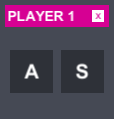
\includegraphics[scale=1]{player1enabledpanel}
\caption*{\hspace*{-0.35cm}R214 G0 B147 A255}
\end{subfigure}
\begin{subfigure}{0.22\textwidth}
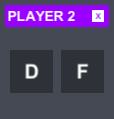
\includegraphics[scale=1]{player2enabledpanel}
\caption*{\hspace*{-0.35cm}R153 G0 B255 A255}
\end{subfigure}
\begin{subfigure}{0.22\textwidth}

\includegraphics[scale=1]{player3enabledpanel}
\caption*{\hspace*{-0.35cm}R51 G153 B255 A255}
\end{subfigure} \\
\begin{subfigure}{0.22\textwidth}
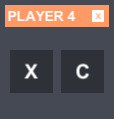
\includegraphics[scale=1]{player4enabledpanel}
\caption*{\hspace*{-0.351cm}R255 G153 B102 A255}
\end{subfigure}
\begin{subfigure}{0.22\textwidth}
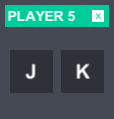
\includegraphics[scale=1]{player5enabledpanel}
\label{fig:b}
\caption*{\hspace*{-0.35cm}R0 G204 B153 A255}
\end{subfigure}
\begin{subfigure}{0.22\textwidth}
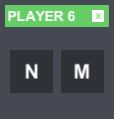
\includegraphics[scale=1]{player6enabledpanel}
\label{fig:b}
\caption*{\hspace*{-0.35cm}R102 G255 B102 A255}
\end{subfigure}
\caption{PlayerEnabledPanel}
\end{figure}

\noindent All of the componetns has its default values hardcoded. All of them are explained in the \hyperref[gui-implementation]{implementation} section.

\subsubsection*{ArenaSizePanel}\label{gui-arenasizepanel}
\indent The \verb+ArenaSizePanel+ background color is exactly the same as the color of the \cprotect{\hyperref[gui-playerenabledpanel]}{\verb|PlayerEnabledPanel|}. The panel itself contains two main components. The first one is a \verb+Panel+ with the background color the same as the color of the \cprotect{\hyperref[gui-playerssettingspanel]}{\verb|PlayersSettingsPanel|}. This panel contains a "ARENA SIZE" \verb+Text+ of a white color written in capitals letters only. The second element of area panel is \verb+Slider+ of the following possible colors:
\begin{figure}[h] 
\centering
\begin{subfigure}{0.22\textwidth}

\includegraphics[scale=1]{slider0}
\caption*{\hspace*{0.1cm}R255 G255 B255 A255}
\end{subfigure}
\begin{subfigure}{0.22\textwidth}

\includegraphics[scale=1]{slider1}
\caption*{\hspace*{0.1cm}R0 G255 B153 A255}
\end{subfigure}
\caption{Slider}
\end{figure}

\noindent The whole component looks as follows:
\begin{figure}[h] 
\centering
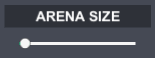
\includegraphics[scale=1]{arenasizepanel}
\caption{ArenaSizePanel}
\end{figure}

\noindent The functionality and implemetation of \verb+ArenaSizePanel+ is described in \hyperref[gui-implementation]{implementation} section.

\subsubsection*{InitialSpeedPanel}\label{gui-initialspeedpanel}
\indent The only differece between \verb+InitialSpeedPanel+ and \verb+ArenaSizePanel+ is the text displayed on the panel. In this case it is "PLAYERS SPEED". For detailed info about the colors and components please refer to \cprotect{\hyperref[gui-arenasizepanel]}{\verb+ArenaSizePanel+} section.
\begin{figure}[h] 
\centering

\includegraphics[scale=1]{initialspeedpanel}
\caption{InitialSpeedPanel}
\end{figure}

\subsubsection*{InitialSizePanel}\label{gui-initialsizepanel}
\indent The only differece between \verb+InitialSpeedPanel+ and \verb+ArenaSizePanel+ is the text displayed on the panel. In this case it is "PLAYERS SIZE". For detailed info about the colors and components please refer to \cprotect{\hyperref[gui-arenasizepanel]}{\verb+ArenaSizePanel+} section.
\begin{figure}[!h] 
\centering

\includegraphics[scale=1]{initialsizepanel}
\caption{InitialSizePanel}
\end{figure}

\subsubsection*{StartButton}\label{gui-startbutton}
\indent The color of the "START" \verb+Button+ is the same as the color of the \hyperref[gui-arenasizepanel]{'slider panels'} text panel background. The \verb+Text+ "START" has a pure white color.
\begin{figure}[h]
\centering
\begin{subfigure}{\textwidth}
\centering

\includegraphics[]{startbutton}
\caption*{R69 G73 B84 A255}
\end{subfigure}
\caption{StartButton}
\end{figure}

\subsubsection*{Startup GUI}
\indent Here is an example of a GUI just after the game starts:
\begin{figure}[h] 
\centering
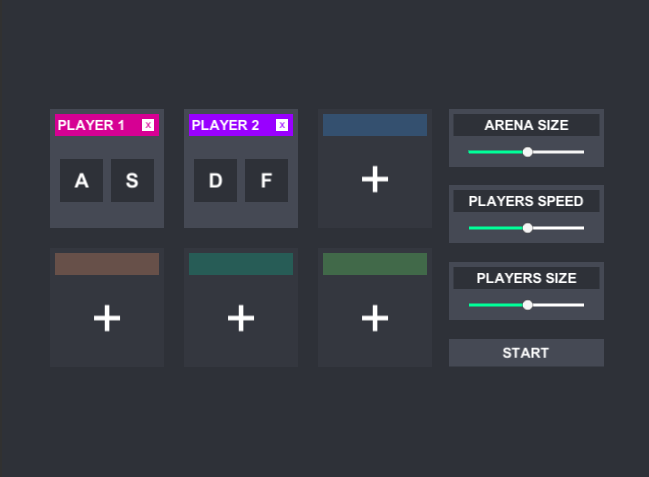
\includegraphics[width=\textwidth]{startupgui}
\caption{Startup GUI}
\end{figure}


\subsubsection{Implemetation}\label{gui-implementation}
\indent The GUI implementation is located in \textit{GUIDataCollector.cs} script. The file is using \textit{Configurator.cs} script to read the initial data and write the user settings before game starts. The following functionalities are implemented:
\begin{itemize}
	\item[-] Adding and Removing player. There is a minimum of two players that must participate the game. There is no possibility  to lower the value from the GUI. A user can manipulate the number of players from two to six. It is also imposible to have more than six players in the game.
	\item[-] Setting the nickname of the player. On each \cprotect{\hyperref[gui-playerenabledpanel]}{\verb+PlayerEnabledPanel+} there is an \verb+InputField+ by witch user can set player unique name. The nickname is limited by 9 characters.
	\item[-] Setting the player movement keys. Each player must have its own movement keys. There is no possibility that two playes has the Setting key set. There is also no possibility that the player has the same key set for both directions.
	\item[-] Changing the initial arena size. The \cprotect{\hyperref[gui-arenasizepanel]}{\verb+ArenaSizePanel+} slider allows user to set the initial arena size. There are three possible sizes of the arena: small, normal and big.
	\item[-] Setting the initial players speed. The \cprotect{\hyperref[gui-initialspeedpanel]}{\verb+InitialSpeedPanel+} slider allows user to set the initial players speed. There are three possible speeds of the players: slow, normal and fast.
	\item[-] Setting the initial players size. The \cprotect{\hyperref[gui-initialsizepanel]}{\verb+InitialSizePanel+} slider allows user to set the initial players size. There are three possible sizes of the players: thin, normal and fat.
	\item[-] Starting the game. The \cprotect{\hyperref[gui-startbutton]}{\verb+StartButton+} loads a new scene with the game itself.
\end{itemize} 

\subsubsection{Sounds}
\indent There are no sounds implemented on the GUI yet.